\subsection{Simulation d'un exemple physique simple}
Prenons un exemple physique simple pour avoir une idée de comment l'algèbre linéaire peut être utilisée dans une simulation.
%
Disons que nous souhaitons simuler une colonne remplie d'huile.
%
Nous connaissons la densité de l'huile contenue dans la colonne : $\rho = 0.9192~kg/m^3$.
%
Nous connaissons aussi l'équation physique de la pression hydrostatique :
%
\begin{equation}
\label{eq:hydrostatic}
\frac{\mathrm d P}{\mathrm d z} = \rho{}g
\end{equation}
%
Dans l'équation~\eqref{eq:hydrostatic}, $P$ désigne la pression, $z$ la profondeur et $g$ l'accélération gravitationnelle.
%
En utilisant le théorème de Taylor au premier ordre, on obtient l'équation :
%
\begin{equation}
P(z_0+h) = P(z_0) + h \frac{\mathrm d P}{\mathrm d z} (z_0) + o(h^2)
\end{equation}
\begin{equation}
\frac{\mathrm d P}{\mathrm d z} (z_0) = \frac{P(z_0+h) - P(z_0)}{h} + o(h^2)
\end{equation}

%   (-_-)   %
\begin{figure}[!ht]
  \centering
  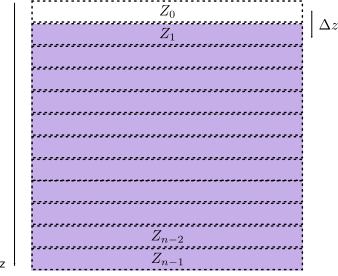
\includegraphics[width=0.5\textwidth]{oil_column}
  \caption{Schéma de la colonne d'huile, il s'agit d'une discrétisation en $n$ cellules et le centre de chaque cellule est séparé d'une distance $\Delta{z}$.}
  \label{fig:oil_schema}
\end{figure}
%
On discrétise le problème en $n$ cellules avec la méthode des différences finies (fig.~\ref{fig:oil_schema}) : considérons $Z_i$ l'approximation de $z$ sur la cellule $i$, $i$ allant de $0$ à $n-1$.
%
Chaque cellule est séparée d'une distance $h$ appelée $\Delta{z}$ :
%
\begin{equation}
\label{eq:taylor_fd}
\frac{\mathrm d P}{\mathrm d z}(Z_i) \approx \frac{P(Z_{i}) - P(Z_{i-1})}{\Delta{z}}
\end{equation}
%
L'injection de \eqref{eq:taylor_fd} dans \eqref{eq:hydrostatic} conduit à :
%
\begin{equation}
\frac{P(Z_{i}) - P(Z_{i-1})}{\Delta{z}} = \rho{}g
\end{equation}
\begin{equation}
\label{eq:system_pressure}
P(Z_{i}) - P(Z_{i-1}) = \rho{}g\Delta{z}
\end{equation}
Nous avons aussi la condition limite qu'à la profondeur 0, la pression est de 1000~hPa ou $10^5$~Pa:
%
\begin{equation}
P(Z_0) = 10^5
\end{equation}
%
Nous pouvons donc écrire le système entier sous la forme d'une matrice à $n$ lignes :
%
\begin{equation}
\label{eq:ax_b}
\begin{bmatrix}
   1   &    0   &    0   & \cdots & \cdots & \cdots & \cdots &   0    \\
  -1   &    1   &    0   & \ddots &        &        &        & \vdots \\
   0   &   -1   &    1   &    0   & \ddots &        &        & \vdots \\
\vdots & \ddots & \ddots & \ddots & \ddots & \ddots &        & \vdots \\
\vdots &        & \ddots & \ddots & \ddots & \ddots & \ddots & \vdots \\
\vdots &        &        & \ddots &   -1   &    1   &    0   &   0    \\
\vdots &        &        &        & \ddots &   -1   &    1   &   0    \\
   0   & \cdots & \cdots & \cdots & \cdots &    0   &   -1   &   1    \\
\end{bmatrix}
\begin{pmatrix}
  P(Z_0)  \\
  P(Z_1)  \\
\vdots \\
\vdots \\
\vdots \\
\vdots \\
P(Z_{n-2}) \\
  P(Z_{n-1})  \\
\end{pmatrix}
=
\begin{pmatrix}
 10^5  \\
\rho{}g\Delta{z}     \\
\vdots \\
\vdots \\
\vdots \\
\vdots \\
\rho{}g\Delta{z} \\
\rho{}g\Delta{z}    \\
\end{pmatrix}
\end{equation}
En faisant la multiplication de chaque ligne de $A$ par $x$, nous obtenons exactement le système d'équations \eqref{eq:system_pressure}.
%
Maintenant que nous avons une matrice $A$ multipliée par un vecteur $x$ égale à un vecteur $b$, il est temps de parler d'algèbre linéaire.
